\documentclass[singlecolumn, 11pt]{revtex4-1}
\usepackage{graphicx}
\usepackage{subfigure}
\usepackage{amsthm}
\usepackage{amssymb}
\usepackage{amsmath}
\usepackage{eucal}
\usepackage{hyperref}
\usepackage{float}
\DeclareGraphicsRule{.tif}{png}{.png}{`convert #1 `dirname #1`/`basename #1 .tif`.png}

%in equations
\newcommand{\dee}[2]{\frac{ \mathrm{d}#1 }{ \mathrm{d}#2 } }
\newcommand{\deedee}[2]{\frac{ \mathrm{d}^2 #1 }{ \mathrm{d} #2^2 } }
\newcommand{\pd}[2]{\frac{\partial#1}{\partial#2}}
%inline
\newcommand{\indee}[2]{\dfrac{ \mathrm{d}#1 }{ \mathrm{d}#2 } }
\newcommand{\indeedee}[2]{\dfrac{ \mathrm{d}^2 #1 }{ \mathrm{d} #2^2 } }
\newcommand{\inpd}[2]{\dfrac{\partial#1}{\partial#2}}
%bold vector
\newcommand{\ve}[1]{\mathbf{#1}}
\newcommand{\gve}[1]{\boldsymbol{#1}}

\begin{document}

\title{LIGO SURF Report: Visualization of images distorted by black holes}

\author{Darius Bunandar \\ Mentors: Mark Scheel and Nick Taylor}

\affiliation{TAPIR Group, Division of Physics, Mathematics, and Astronomy, California Institute of Technology, CA 91125, USA}

\date{\today}

\begin{abstract}
One of the most promising sources of gravitational waves for potential detection by LIGO is the inspiral and merger of two black holes. In an effort to aid LIGO data analysis, the Caltech-Cornell SXS collaboration is numerically solving Einstein's equations for a number of such binary black hole systems with varying mass ratios and spins. In this project, we investigate a novel way to visualize the structure of such a numerical solution by producing images of a distorted stellar background in the vicinity of black holes. This involves following the paths of photons through regions of strong gravitational field�produced by the black holes�from the observer to the light sources at distant locations in the background. In this work, we present some distorted images of single as well as binary black hole systems.
\end{abstract}

\maketitle

\section{Introduction}
\label{sec:introduction}
Consider an observer taking a picture of the night sky using a pinhole camera with one or more black holes present in the vicinity.
The image of the night sky that is seen by the observer will be distorted because the black hole(s) curves the spacetime in the region---bending the paths of the light rays originating from the stars in the night sky.
Fig. \ref{fig:raytracing} presents an example of this scenario with the observer pointing its pinhole camera at a system of binary black holes.
Here we emphasize that we not only need the image of the night sky behind the black hole(s) as viewed by the observer, but we also need the night sky seen by the observer's \emph{entire} celestial sphere. Some of the light rays originating from behind the observer might be hurled back towards the observer by the black holes' strong gravitational field, as shown in the figure.

\begin{figure}[!htp]
   \centering
   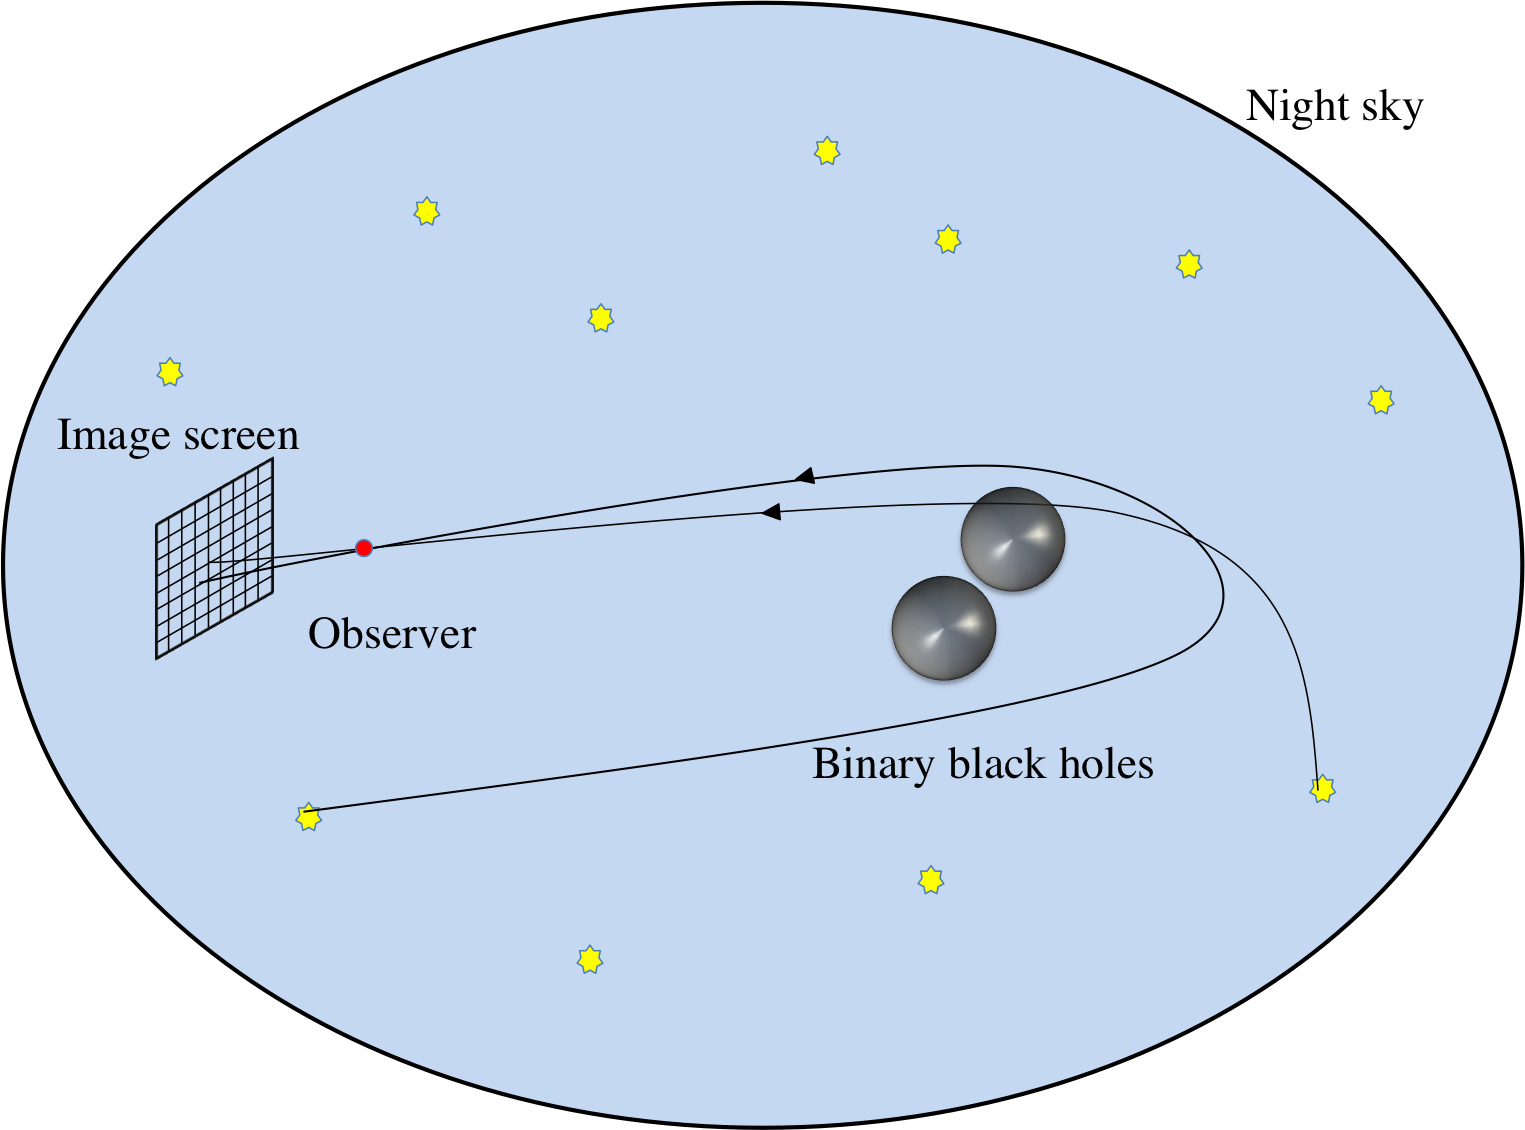
\includegraphics[width=.6\textwidth]{raytracing.png} % requires the graphicx
   \caption{A schematic of gravitational lensing of light rays originating from the stars in the night sky. The bending of light is caused by the strong gravitational field produced by the colliding binary black holes.}
   \label{fig:raytracing}
\end{figure}

The image seen by an observer---holding a pinhole camera---is the image formed by tracing the path of light \emph{backwards in time} from the observer through each pixel on the pinhole camera image screen.
Some of these light rays may trace back to the black holes' event horizons and the observer would see these pixels as black (since no light would have been emitted from there); some of the light rays may trace back to the background night sky, and these are the parts of night sky seen by the observer.

We are developing a computer code capable of tracing the paths of light rays through any spacetime---even when the metric is not analytic or when the gravitational field produced by the black hole(s) is exceptionally strong. Although similar work making use of analytical expressions has already been done \cite{krawisz, lindner, shadows}, what is novel about our code is that it will be able to use numerically computed dynamical spacetimes---not just analytical spacetimes. A recent work to view collapsing neutron stars has also been done in Ref. \cite{gyoto}. Ultimately, we would like the code to be perform well when the image is being distorted by interesting astronomical phenomena: collision of binary black holes, collision of two neutron stars forming a black hole, and even a neutron star falling into a black hole. A neutron star would not only bend the light rays originating from the other stars in the night sky, but also emit its own light.

\section{Null Geodesic Equations}
\label{sec:nullgeodesic}

We approach the problem by integrating the geodesic equation for photons backwards in time: integrating from the observer back to the source. The uniqueness of the path of every single photon arriving at the observer allows us to do so. We plan to follow the geodesic integration method commonly used in event horizon finders \cite{scheel, shapiro, hughes, anninos, libson}.

Consider a single photon arriving at the observer; the geodesic equation for a photon is:
\begin{equation}
\label{eq:geodesic}
\deedee{x^{\mu}}{\lambda} + \Gamma^{\mu}_{\; \alpha \beta} \dee{x^{\alpha}}{\lambda} \dee{x^{\beta}}{\lambda} = 0,
\end{equation}
where $x^{\mu}$ is the position of the photon along the geodesic, $\lambda$ is the affine parameter for the photon. $\Gamma^{\mu}_{\phantom{a} \alpha \beta}$ is the Christoffel symbol, which can be computed from the metric $g_{\mu \nu}$ and its partial derivatives:
\begin{equation}
\Gamma^{\mu}_{\phantom{a} \alpha \beta} = \frac{1}{2} g^{\mu \nu} \left( g_{\nu \alpha , \beta} + g_{\nu \beta , \alpha} - g_{\alpha \beta, \nu}\right).
\end{equation}

We can then convert Eq. \ref{eq:geodesic} to a system of two first-order linear ordinary equations by defining velocity $p^i \equiv \indee{x^i}{t}$; allowing us to obtain:
\begin{align}
\label{eq:old}
\dee{{x}^{i}}{t} &= p^i , \nonumber \\
\dee{{p}^{i}}{t} &= \left( \Gamma^{0}_{\phantom{a} \nu \delta} p^i - \Gamma^{i}_{\; \nu \delta} \right) p^{\nu} p^{\delta}.
\end{align}
Here we use greek indices to denote spacetime components---0, 1, 2, 3---and the latin indices to denote only spatial components: 1, 2, 3. Details on deriving Eq. \ref{eq:old} can be found in Ref. \cite{scheel}.

Nevertheless, such na\"{i}ve formulation has shown to propagate large errors numerically, particularly from calculating the Christoffel symbols. It is always necessary to interpolate the values of the metric and their derivatives to the \emph{spacetime} location of the photons, resulting in significant numerical errors. It can be shown that the size of the numerical errors in integrating the null geodesic equation scales with the number of metric terms used in the integration \cite{bohn}. The formulation described by Eq. \ref{eq:old} uses many metric terms and its derivatives in calculating the Christoffel symbols, shown explicitly below:
\begin{align}
\Gamma^0_{\phantom{0}00} &= \frac{1}{\alpha} \left( \alpha_{,t} + \beta^k \alpha_{,k} - K_{ij} \beta^i \beta^j \right), \nonumber \\
\Gamma^k_{\phantom{0}00} &= \gamma^{kj} \left[ \beta_{j,t} + \alpha \alpha_{,j} - \frac{1}{2} \left( \gamma_{mn} \beta^m \beta^n \right)_{,j} \right] - \beta^k \Gamma^0_{\phantom{0}00}, \nonumber \\
\Gamma^0_{\phantom{0}i0} &= \frac{1}{\alpha} \left( \alpha_{,i} - K_{ij} \beta^j \right), \nonumber \\
\Gamma^k_{\phantom{0}i0} &= -\alpha K_{i}^{\phantom{i} k} + ^{(3)}\nabla_i \beta^k - \Gamma^{0}_{\phantom{0}i0} \beta^k, \nonumber \\
\Gamma^0_{\phantom{0}ij} &= - \frac{1}{\alpha} K_{ij}, \nonumber \\
\Gamma^k_{\phantom{0}ij} &= ^{(3)}\Gamma^k_{\phantom{0}ij} + \frac{K_{ij}}{\alpha} \beta^k.
\end{align}
where $\alpha$ and $\beta^i$ are the lapse and shift functions respectively. $\gamma_{ij} = g_{ij}$ is the spatial three-metric and $\gamma^{ij} = \left( \gamma_{ij} \right)^{-1} = g^{ij} + \dfrac{\beta^i \beta^j}{\alpha^2}$ is its inverse. $K_{ij}$ is the extrinsic curvature defined as:
\begin{equation}
K_{ij} = \frac{1}{2\alpha} \left( - \dot{\gamma}_{ij} + 2 \gamma_{ik} \beta^k_{\phantom{k},j} + \gamma_{ij,m} \beta^m \right).
\end{equation}
We would expect a formulation with fewer metric terms to have smaller errors.

Alternatively, we can reduce the number of metric terms and its derivatives required to integrate the null geodesic by defining the photon's velocity in terms of its affine parameter:
\begin{equation}
p^i = \dee{x^i}{\lambda}.
\end{equation}
We can then obtain a similar system of first-order non-linear ODEs by noticing that for a null geodesic $p^0 = \dfrac{1}{\alpha} \sqrt{\gamma^{ij} p_i p_j} = \indee{t}{\lambda}$, as shown below:
\begin{align}
\label{eq:hughes}
\dee{x^i}{t} &= \gamma^{ij} \: \frac{p_j}{p^0} - \beta^i, \nonumber \\
\dee{p_i}{t} &= - \alpha \alpha_{,i} p^0 + \beta^k_{\phantom{b},i} p_k - \frac{1}{2} \gamma^{jk}_{\phantom{ab} ,i} \frac{p_i p_k}{p^0}.
\end{align}
Details of the derivation can be found in Ref. \cite{hughes} by Hughes \emph{et al.}. The formulation above requires fewer metric terms than the one describe by Eq. \ref{eq:old}. In addition, the formulation does not require the time derivative of any metric component---making it a prime candidate for null geodesic integration. However, the value of $p^0$ blows up as one integrates backwards in time especially very near the event horizon of a black hole causing the evolution of a geodesic near a black hole to be very slow compared to geodesics located far from any black hole.

If we then normalize Eq. \ref{eq:hughes} by defining $\Pi_i = p_i /(\alpha p^0)$, we would have a much more consistent evolution of a null geodesic, be it located near the black hole or not. The new evolution equations are:
\begin{align}
\label{eq:normalized}
\dee{x^i}{t} &= \alpha \Pi^i - \beta^i, \nonumber \\
\dee{\Pi_i}{t} &= -\alpha_{,i} + \alpha_{,j} \Pi^j - \alpha K_{jk} \Pi^j \Pi^k \Pi_i - \frac{\alpha}{2} \gamma^{jk}_{\phantom{ab},i} \Pi_j \Pi_k,
\end{align}
where the lapse function $\alpha$ is used in the definition of $\Pi_i$ to reduce the number of terms in the equation.

This new formulation is a compromise between the two previous formulations. While it does have more metric terms than the formulation in Eq. \ref{eq:hughes} along with a term (the extrinsic curvature) involving the time derivative of the metric, the absence of $p^0$ ensures that evolution does not exponentially slow down near a black hole. This new formulation has also been shown to have a smaller fractional error compared to the ``na\"{i}ve'' formulation (Eq. \ref{eq:old}) when used to find the event horizon of a spinning black hole \cite{bohn}.

\section{Initial Conditions}

In this section, we outline the method we use to initialize the photons' momenta and positions.
Here, we again note that we are evolving the photons backwards in time which means that what we are initializing is in fact the photons' final momenta and positions.
Since the geodesic equations are a system of two first-order non-linear ordinary differential equations, only two initial conditions�the photons' final momenta and positions�are necessary to obtain a unique solution to the system of equations.

The photons' final positions are the camera position because all the photons have to reach the camera simultaneously for us to form an image.
The photon momenta, on the other hand, are initialized by considering the pixel that the photon travels to when forming the image.
To do so, we must first specify the directions that the camera is pointing and this can be done by defining three different vectors:
\begin{enumerate}

\item $v^i = \indee{x^i}{t}$, which is the three--velocity of the camera with respect to some arbitrary coordinate system---the same coordinate system in which we express the metric components. We call this coordinate system the 'inertial frame' because in this frame the spatial geometry asymptotically approaches Cartesian at spatial infinity.
We can then determine the four-velocity of the camera $(U^{\mu} = \indee{x^\mu}{\tau} )$ using the relation: $g_{\mu \nu} U^{\mu} U^{\nu} = (U^0)^2  \left( g_{\mu \nu}  v^{\mu} v^{\nu} \right) = -1$.
In this relation we have used the definition $U^{\mu} = U^0 v^{\mu}$, where $U^0 = \indee{t}{\tau}$ and $\tau$ is the proper time.

\item $\pi^i$ which is the three--momentum of the photon going through the center pixel in the inertial frame.
Similarly, we can determine the four-momentum of the photon $(\pi^{\mu})$ by ensuring that the four-momentum is null, i.e. $g_{\mu \nu} \pi^{\mu} \pi^{\nu} = 0$.

\item $\xi^i$ which is the upwards direction of the camera in the inertial frame.
We define that its zeroth component, $\xi^0 = 0$ in the inertial frame.
\end{enumerate}

Next, we define the vector $r^{\mu}$ which is the direction that the camera is pointing by a Gram-Schmidt process:
\begin{equation}
r^{\mu} = \pi^{\mu} + (\gve{\pi} \cdot \ve{U}) U^{\mu},
\end{equation}
which can then be normalized: $\hat{r}^{\mu} = r^{\mu} / \sqrt{\ve{r} \cdot \ve{r} }$. 
Notice that 
\begin{equation}
\ve{r} \cdot \ve{U} = 0, 
\end{equation}
which means that the vector $r^{\mu}$ is a purely spatial vector in the frame which is co-moving with the camera because $U^{\mu} \rightarrow (1,0,0,0)$ in this frame.
We then define the vector $\zeta^{\mu}$ which is the upwards direction of the camera in the camera's co-moving reference frame (CMRF) by the following relations:
\begin{equation}
\bar{\zeta}^{\mu} = \xi^{\mu} + ( \gve{\xi} \cdot \ve{U}) U^{\mu}
\end{equation}
and
\begin{equation}
\zeta^{\mu} = \bar{\zeta}^{\mu} - ( \gve{\bar{\zeta}} \cdot \ve{\hat{r}} ) \hat{r}^{\mu}.
\end{equation}
These two relations give us the properties: $\gve{\zeta} \cdot \ve{U} = 0$ and $\gve{\zeta} \cdot \ve{r} = 0$. 
Similarly, $\gve{\zeta}$ can be normalized: $\hat{\zeta}^{\mu} = \zeta^{\mu} / \sqrt{\gve{\zeta} \cdot \gve{\zeta} }$.

Now, notice that with $U^{\mu}$, $\hat{r}^{\mu}$, and $\hat{\zeta}^{\mu}$, we can form an orthonormal tetrad; written explicitly:
\begin{align}
\ve{e}_0^{\phantom{1} \mu} &= U^{\mu}, \nonumber \\
\ve{e}_1^{\phantom{1} \mu} &= \hat{r}^{\mu}, \nonumber \\
\ve{e}_2^{\phantom{1} \mu} &= \hat{\zeta}^{\mu}, \: \:\text{and} \nonumber \\
\ve{e}_3^{\phantom{1} \mu} &= (\ve{e}_1 \times \ve{e}_2)^{\mu} = \varepsilon^{\phantom{\alpha \beta \gamma} \mu}_{\alpha \beta \gamma} \; U^{\alpha} \; \hat{r}^{\beta} \; \hat{\zeta}^{\gamma}.
\end{align}
Let's say we want to calculate the initial momentum of the photon that passes through the pixel $\{a,b\}$, where $a \in [0, 1]$ and $b \in [0, 1]$. $i$ and $j$ are the pixel location in terms of fraction of the image's horizontal and vertical lengths with $\{a,b\} = \{ 0, 0\}$ at the top left corner of the image.
The momentum of the photon in interest is then:
\begin{equation}
p^{\mu}_{\phantom{\mu} (a) (b)} = c \; \ve{e}_0^{\phantom{0} \mu} + \ve{e}_1^{\phantom{0} \mu} - \left( b - \frac{1}{2} \right)\; \ve{e}_2^{\phantom{0} \mu} + \left( a - \frac{1}{2} \right) \; \ve{e}_3^{\phantom{0} \mu},
\end{equation}
where $c = \sqrt{1 + \left( b - 1/2 \right)^2 + \left( a - 1/2 \right)^2}$, found by demanding $p^{\mu} p_{\mu} = 0$.

The Levi-Civita tensor, $\gve{\varepsilon}$, is defined as:
\begin{equation}
\varepsilon_{\alpha \beta \gamma \delta} = \sqrt{-g} \: [\alpha \beta \gamma \delta],
\end{equation}
where
\begin{align}
[\alpha \beta \gamma \delta] = \left\{ \begin{array}{ll}
		+1	&	\mbox{if $\alpha \beta \gamma \delta$ is an even permutation of 0123}, \\
		-1	&	\mbox{if $\alpha \beta \gamma \delta$ is an even permutation of 0123}, \\
		0	&	\mbox{if $\alpha \beta \gamma \delta$ are not all different}. 
		\end{array} \right.
\end{align}
Note that this convention is the one that is defined in Ref. \cite{mtw} and \cite{nichols}.

Notice that when using this method, there is no need to boost any of the vector from the inertial frame to the camera's CMRF and back.
We can simply calculate all the vectors and the photons' momenta in the inertial frame (or any other frame).

\section{Comparison against integration using analytical expressions}

We have produced a single non-spinning black hole image as a check against analytics. For the purpose of clarity, the background image was produced using a grid of gradient color map (see Fig. \ref{fig:gridcolor}) that has undergone cylindrical Plate Car\'{e}e projection. This projection casts the horizontal lines into lines of constant latitude and the vertical lines into lines of constant longitude.

\begin{figure}[!htp]
   \centering
   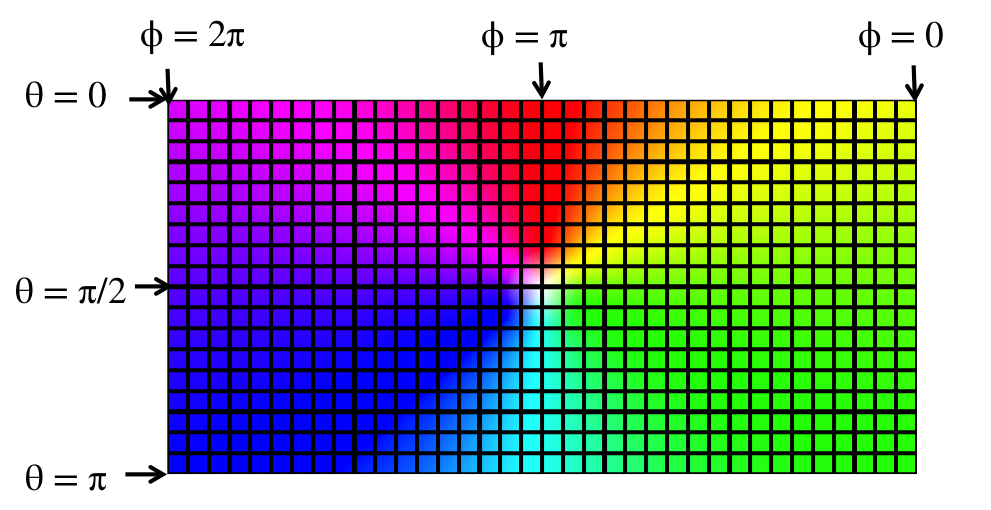
\includegraphics[width=.8\textwidth]{grid_color.png} % requires the graphicx
   \caption{A grid of gradient color map with the projected angular positions of some lines denoted.}
   \label{fig:gridcolor}
\end{figure}

Fig. \ref{fig:schwarzschild} shows the image distorted by a Schwarzschild black hole as seen by an observer located $50$ M away from the hole in Kerr-Schild coordinates. The hole is located at the center of the domain, i.e. $(x, y, z) \rightarrow (0, 0, 0)$, and the observer is placed at the positive $x$-axis, i.e. $(x, y, z) \rightarrow (50, 0, 0)$, looking straight in the negative $x$-axis direction. Our projection convention places the center of the image on the negative $x$-axis; this would correspond to the vertical line $\phi = \pi$ in Fig. \ref{fig:gridcolor}. Moreover, the positive $x$-axis would correspond to both the vertical lines $\phi = 0$ and $\phi = 2\pi$ in Fig. \ref{fig:gridcolor}.

\begin{figure}[H]
   \centering
   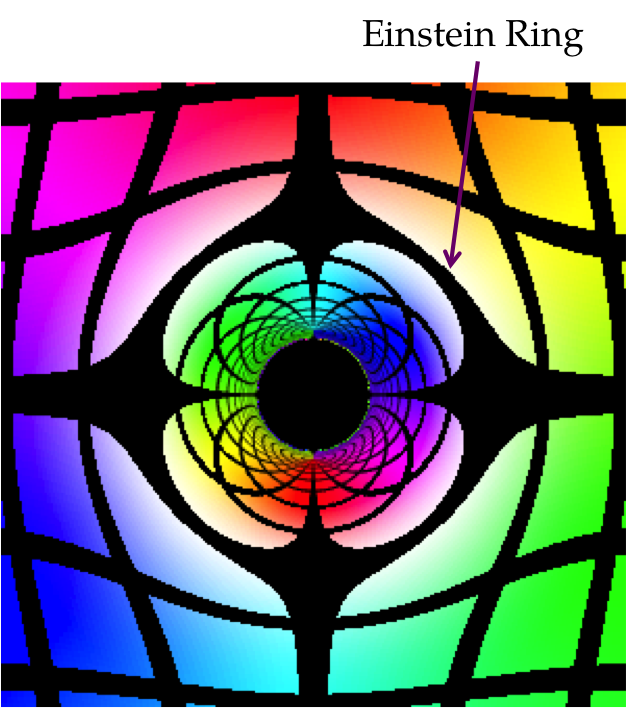
\includegraphics[width=.6\textwidth]{SchSideWithLabel.png} % requires the graphicx
   \caption{An image grid of gradient color map (Fig. \ref{fig:gridcolor}) distorted by a Schwarzschild black hole. The arrow indicates the location of the Einstein ring in the image. The resolution of the observer's pinhole camera is $300 \times 300$ in this case.}
   \label{fig:schwarzschild}
\end{figure}

\newpage
Referring to Fig. \ref{fig:schwarzschild}, the small black circle in the middle of the distorted image is the black hole, i.e. the set of photons that end up on the event horizon when integrated backwards in time from the camera. The large circular-like grid line is the Einstein ring that is produced from a single grid point which is located at the center of Fig. \ref{fig:gridcolor}. It is interesting to note that inside the Einstein ring, the image is not only distorted but also reflected in the sense that light that originates from the right (or up) is seen by the observer as if it has originated from the left (or down). Outside the Einstein ring, no such reflection is apparent although the grid lines do appear distorted.

As a check of our results, we compare the geodesic trajectory in Schwarzschild spacetime from the observer's camera backwards in time obtained by numerically integrating Eq. \ref{eq:normalized} to the trajectory obtained by integrating analytical expressions. When numerically integrating Eq. \ref{eq:normalized}, we use the Kerr-Schild coordinates (same as ingoing Eddington-Finkelstein coordinates):
\begin{equation}
g_{\alpha \beta} = \eta_{\alpha \beta} + \frac{2M}{r} l_{\alpha} l_{\beta},
\end{equation}
where $\eta_{\alpha \beta} = \text{diag}(-1,1,1,1)$ is the Minkowski metric and $l_{\alpha}$ is an outgoing null vector with respect to both the Minkowski and the Schwarzschild metric; the outgoing null vector written explicitly in terms of the coordinates $(t, x, y, z)$ has the form
\begin{equation}
l_{\alpha} \rightarrow \left( 1, \frac{x}{r}, \frac{y}{r}, \frac{z}{r} \right).
\end{equation}
In these coordinates, the quantities $\alpha$ and $\beta_i$ are
\begin{equation}
\alpha^2 = \frac{1}{1+2M/r},
\end{equation}
and
\begin{equation}
\beta^i = -\frac{2M/r}{1+2M/r} x^i,
\end{equation}
where $x^i \rightarrow (x, y, z)$ and when the hole is centered at the origin.

The trajectory obtained using the metric defined above is compared to the trajectory obtained from integrating the following equations of motion \cite{mtw}:
\begin{align}
\label{eq:eom}
\dee{r}{\lambda} &= \pm \sqrt{ \frac{1}{b^2} -  \left( \frac{1 - 2M/r}{r^2} \right)}, \nonumber \\
\dee{\phi}{\lambda} &= \frac{1}{r^2}, \\
\dee{\bar{t}}{\lambda} &= \frac{1}{b (1-2M/r)}, \nonumber 
\end{align}
where $\lambda$ is the affine parameter and the coordinate quantities $\bar{t}$, $r$, and $\phi$ are those of the Schwarzschild coordinates whose line element is:
\begin{equation}
\mathrm{d}s^2 = -\left(1-2M/r \right) \mathrm{d}\bar{t}^2 + \frac{\mathrm{d}r^2}{\left(1-2M/r \right)} + r^2 \left( \mathrm{d}\theta^2 + \sin^2{\theta} \; \mathrm{d}\phi^2 \right).
\end{equation}
$b$ here is the impact parameter defined as:
\begin{equation}
\label{eq:impact}
b = \pm \frac{p_{\phi}}{p_{\bar{t}}}.
\end{equation}
The equations of motion defined in Eqs. \ref{eq:eom} are defined for null geodesics traveling in a polar orbit at the equator $(\theta = \pi/2 )$, which has zero momentum in the $\theta$ direction:
\begin{equation}
p^{\theta} = \dee{\theta}{\lambda} = 0.
\end{equation}
Such choice of $\theta$ is done without any loss of generality because of the spherical symmetry.

Because the numerical simulation is done in Kerr-Schild coordinates, we need to transform the equations of motion in terms of these coordinates. The line element for the Kerr-Schild coordinates is:
\begin{equation}
\mathrm{d}s^2 = -\left(1-\frac{2M}{r} \right) \mathrm{d}t^2 + \frac{4M}{r} \mathrm{d}r \mathrm{d}t + \left(1+ \frac{2M}{r} \right) \mathrm{d}r^2 + r^2 \left( \mathrm{d}\theta^2 + \sin^2{\theta} \; \mathrm{d}\phi^2 \right).
\end{equation}
From the expressions of the Schwarzschild metric in the two coordinate systems, it is clear that the area coordinate $r$ and the angular coordinates $(\theta, \phi)$ in the Kerr-Schild coordinates are the same as those in the Schwarzschild coordinates. From the two line elements alone, we can obtain the relationship between the two coordinate systems:
\begin{equation}
\label{eq:kssch}
\mathrm{d}\bar{t} = \pm \left( \mathrm{d}t - \frac{2M/r}{1-2M/r} \mathrm{d}r \right ).
\end{equation}
Using this relationship we can then cast the equations of motion described by Eqs. \ref{eq:eom} in terms of the Kerr-Schild time instead of the affine parameter $\lambda$.

We then proceed by choosing the direction of time in both coordinates to be in the same direction as the affine parameter. This implies the choice of positive signs in the impact parameter (Eq. \ref{eq:impact}) and in the relationship between $\bar{t}$ and $t$ (Eq. \ref{eq:kssch}). Because we are integrating backwards in time, the choice of sign in $\indee{r}{\lambda}$ is positive initially when the photon initially approaches the hole. After the photon has reached its distance of closest approach, the sign in $\indee{r}{\lambda}$ would then be negative to signify the photon traveling away from the hole. The distance of closest approach, $R$, can be found by solving for $r$ when $\indee{r}{\lambda}= 0$; written in implicit form:
\begin{equation}
\frac{R^2}{1-2M/R} = b^2.
\end{equation}
Obtaining analytical expressions or $r (t)$ and $\phi (t)$ are exceptionally difficult generally. We therefore integrated the equations of motion using numerical means. Our choice of integrator was the Dormand-Prince method.

Here we present plots comparing the trajectories of two photons: one that originates from the night sky and one that (potentially) originates from the black hole.
\begin{figure}[H]
\centering
	\subfigure[Plot of the area coordinate $r$ vs. Kerr-Schild time $t$.]{
		\label{fig:RvsT}
		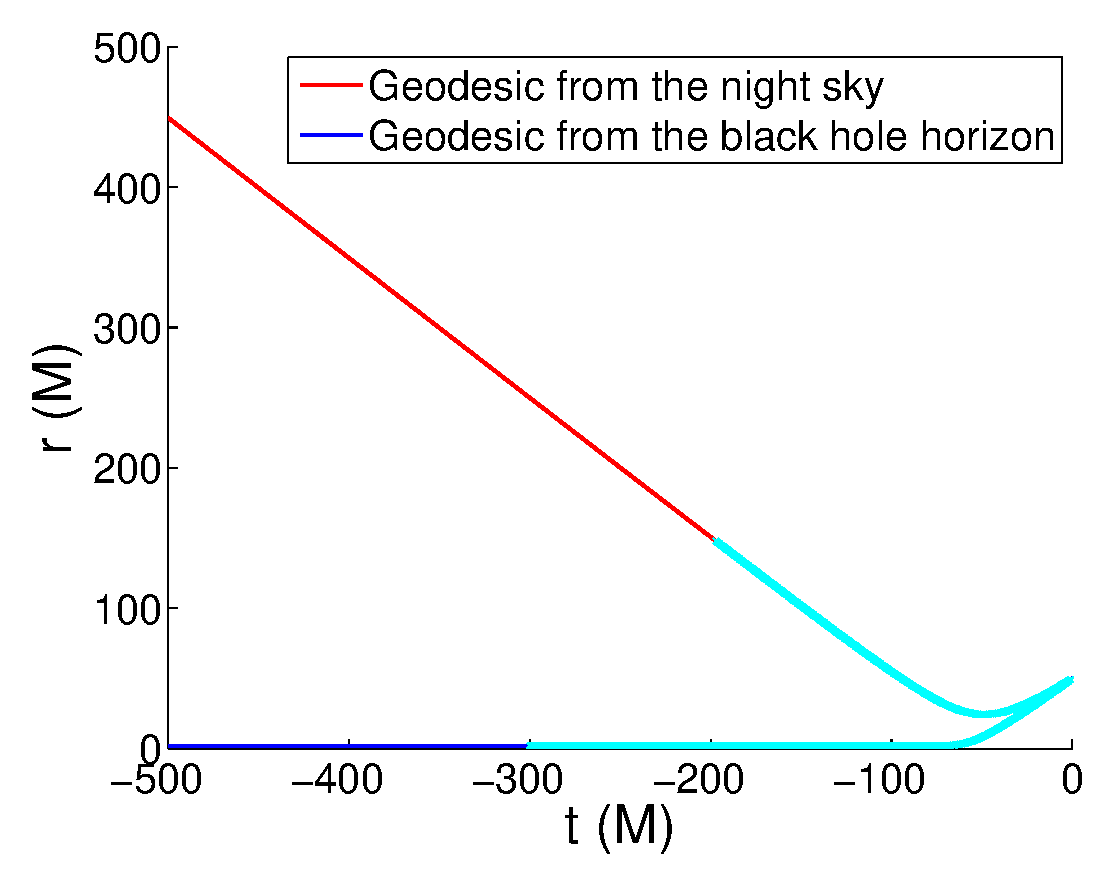
\includegraphics[width=.48\textwidth]{RvsT.eps}
		}
	\subfigure[Plot of the angular coordinate $\phi$ vs. Kerr-Schild time $t$.]{
		\label{fig:PhivsT}
		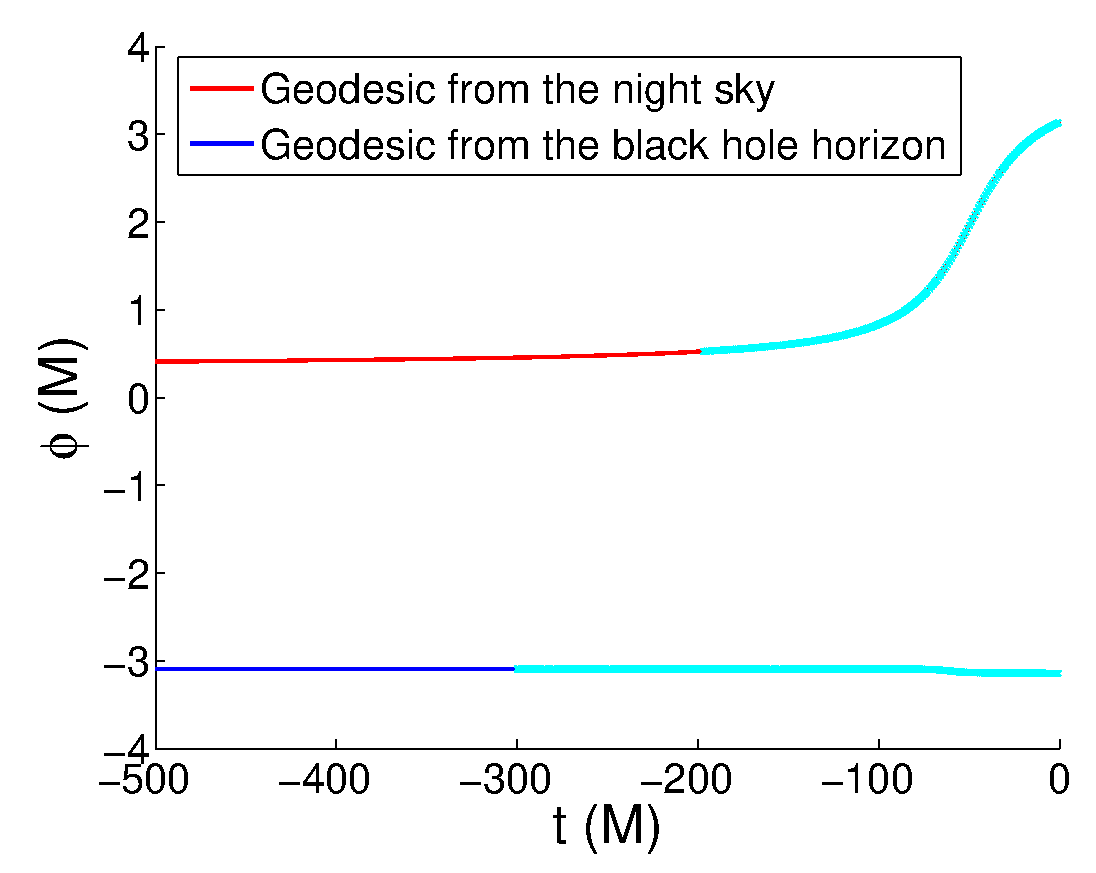
\includegraphics[width=.48\textwidth]{PhivsT.eps}
		}
	\subfigure[Plot of the difference in the area coordinate $r$ between the one obtained using Eqs. \ref{eq:eom} and Eqs. \ref{eq:normalized}.]{
		\label{fig:dRvsT}
		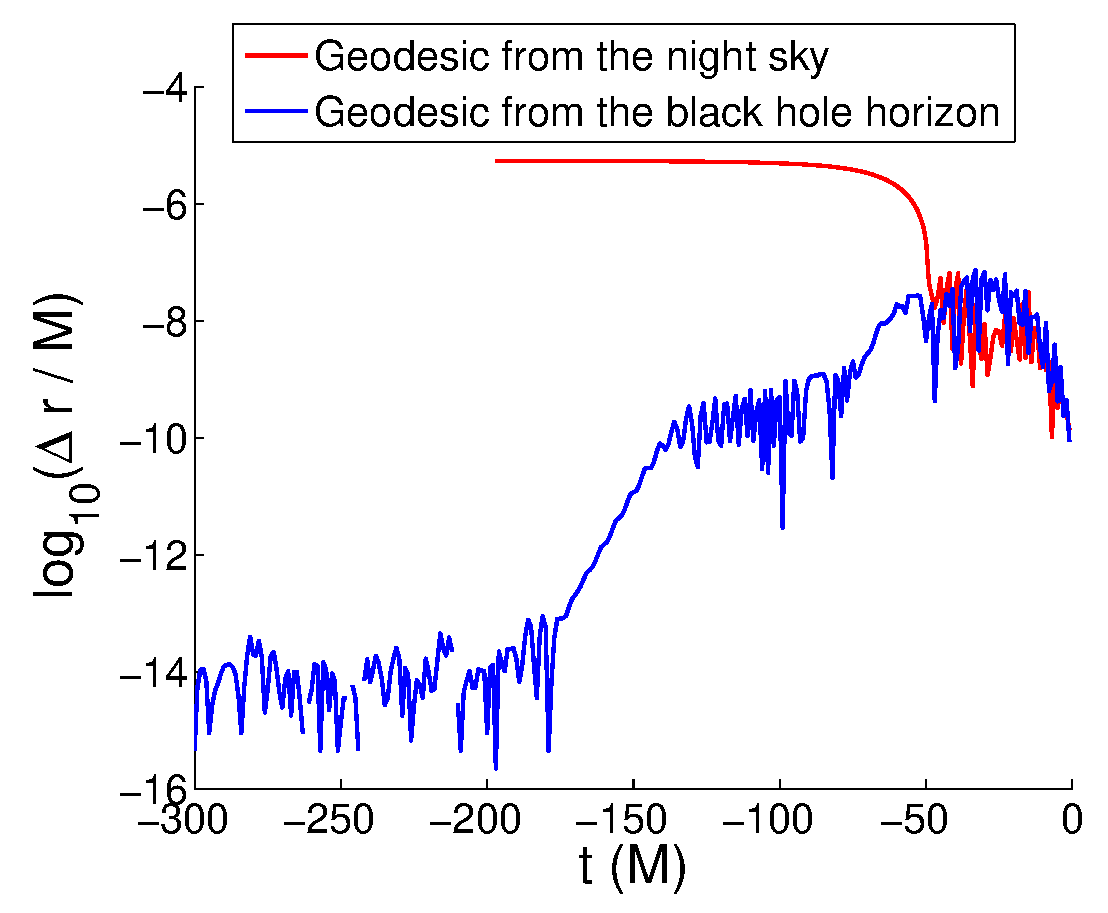
\includegraphics[width=.48\textwidth]{DRvsT.eps}
		}
	\subfigure[Plot of the difference in the angular coordinate $\phi$ between the one obtained using Eqs. \ref{eq:eom} and Eqs. \ref{eq:normalized}.]{
		\label{fig:dPhivsT}
		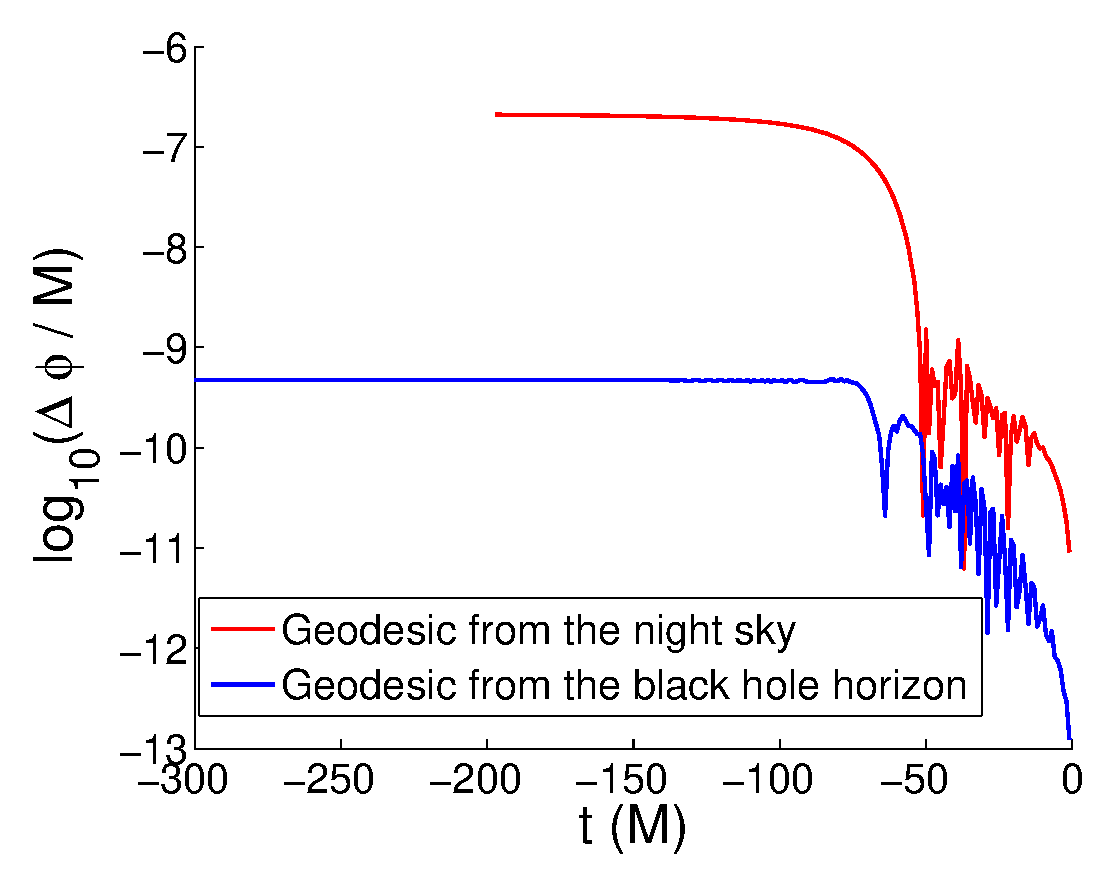
\includegraphics[width=.48\textwidth]{DPhivsT.eps}
		}
	\caption{Plots comparing the trajectories of two photons: one that originates from the night sky (red) and one that (potentially) originates from the black hole (blue). The light blue points are those that are obtained from the Eqs. \ref{eq:normalized}.}
\end{figure}

\newpage
Referring to Figs. \ref{fig:dRvsT} and \ref{fig:dPhivsT}, we can see that the difference between the two results shot up at around $t \approx -50$ M for the photon that originates from the night sky. We believe that the huge increase in the difference between the two results were caused when we had to change the sign of the equation for $\indee{r}{\lambda}$ right when the photon reaches its distance of closest approach. We believe that the change in the sign of $\indee{r}{\lambda}$ was not made at exactly the right time causing the drastic increase in errors. The difference between the two results then plateaus right after this turning point. Nevertheless, considering that both independent results were obtained using numerical integration, we believe that the small difference between the two results means that they agree well with each other.

\section{Single Black Hole Images}

Figs. \ref{fig:side_0}--\ref{fig:side_4} and \ref{fig:top_0}--\ref{fig:top_4} are side and top-down views of a single black hole with different spins. The black holes spin $(a)$ are pointing in the positive $z$-direction. 

Similar to Fig. \ref{fig:schwarzschild}, the the hole is located at the center of the domain and the observer is placed 50 M away in Kerr-Schild coordinates. For the side view (Figs. \ref{fig:side_0}--\ref{fig:side_4}), the observer is placed at the positive $x$-axis, i.e. $(x,y,z) \rightarrow (50,0,0)$. For the top-down view (Figs. \ref{fig:top_0}--\ref{fig:top_4}), the observer is placed at the $z$-axis, i.e. $(x,y,z) \rightarrow (0,0,50)$.

\begin{figure}[!htp]
\centering
	\subfigure[$a = 0.0000$ M.]{
		\label{fig:side_0}
		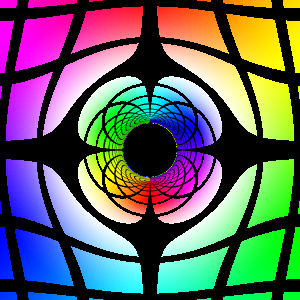
\includegraphics[width=.4\textwidth]{Side_0.png}
		}
	\subfigure[$a = 0.2510$ M.]{
		\label{fig:side_1}
		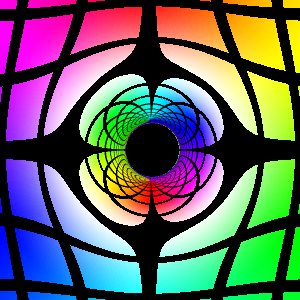
\includegraphics[width=.4\textwidth]{Side_1.png}
		}
	\subfigure[$a = 0.5035$ M.]{
		\label{fig:side_2}
		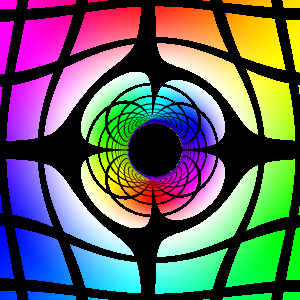
\includegraphics[width=.4\textwidth]{Side_2.png}
		}
	\subfigure[$a = 0.7478$ M.]{
		\label{fig:side_3}
		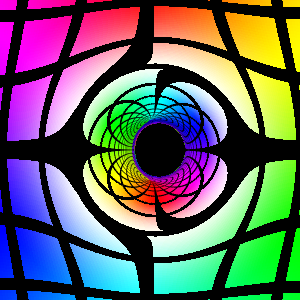
\includegraphics[width=.4\textwidth]{Side_3.png}
		}
	\subfigure[$a = 0.9999$ M.]{
		\label{fig:side_4}
		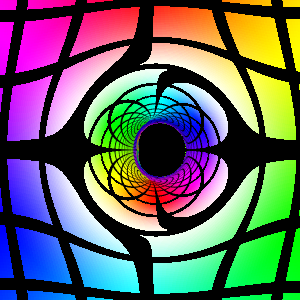
\includegraphics[width=.4\textwidth]{Side_4.png}
		}
	\caption{Side view images of the gradient color map (Fig. \ref{fig:gridcolor}) distorted by single black hole with different spins. The resolution of the observer's pinhole camera is $300 \times 300$.}
\end{figure}

\begin{figure}[!htp]
\centering
	\subfigure[$a = 0.0000$ M.]{
		\label{fig:top_0}
		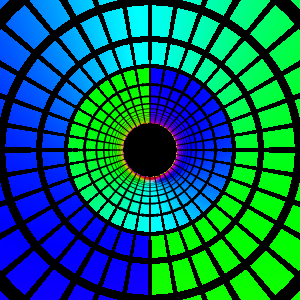
\includegraphics[width=.4\textwidth]{Top_0.png}
		}
	\subfigure[$a = 0.2510$ M.]{
		\label{fig:top_1}
		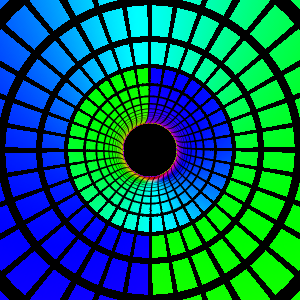
\includegraphics[width=.4\textwidth]{Top_1.png}
		}
	\subfigure[$a = 0.5035$ M.]{
		\label{fig:top_2}
		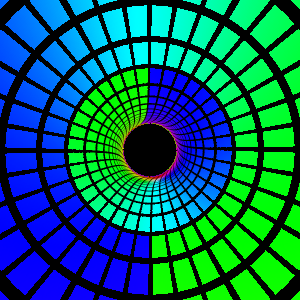
\includegraphics[width=.4\textwidth]{Top_2.png}
		}
	\subfigure[$a = 0.7478$ M.]{
		\label{fig:top_3}
		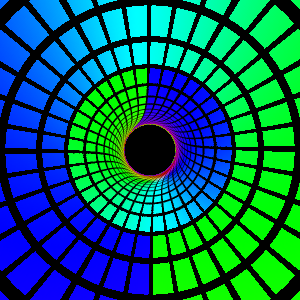
\includegraphics[width=.4\textwidth]{Top_3.png}
		}
	\subfigure[$a = 0.9999$ M.]{
		\label{fig:top_4}
		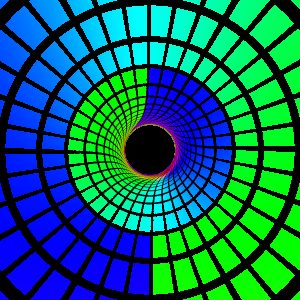
\includegraphics[width=.4\textwidth]{Top_4.png}
		}
	\caption{Top-down view images of the gradient color map (Fig. \ref{fig:gridcolor}) distorted by single black hole with different spins. The resolution of the observer's pinhole camera is $300 \times 300$.}
\end{figure}

The effects of frame-dragging due to the spin of the black hole are obvious in these figures. Referring to Figs. \ref{fig:side_0}--\ref{fig:side_4}, frame-dragging causes the black hole to shift to the right. Inside the Einstein ring, since the hole's spin is pointing upwards, the photons that make up the image to the right side of the hole have to travel for a longer amount of affine parameter than those that make up the image to the left side of the hole. As a result, the geodesic trajectories for the photons that make up the image to the right side of the hole are bent at larger angles than those that make up the image to the left side of the hole. Moreover, the perfectly circular Einstein ring in the Schwarzschild hole case is distorted due to frame-dragging.

Referring to Figs. \ref{fig:top_0}--\ref{fig:top_4}, frame-dragging causes a tangential distortion to the longitudinal lines in the same direction of the spin (out of the page). 
Here we note that in this top-down view, the bright red ring right outside of the hole is produced by geodesics that have traveled from behind the observer.
We also note that the sudden transition between the blue and green color was caused by the way we project our background image.

\newpage
\section{Equal Mass Binary Black Hole Images}
The simulation of binary black hole inspiral and coalescence has been one of the most important achievements of numerical relativity. As of now, there is no analytical expression for the spacetime produced by compact binary black hole merger.

In this section we present images of an equal-mass non-spinning binary black hole system at different times before merger (as seen by the observer). Similar to the single black hole cases, we place our observer 50 M away from the origin in the positive $x$-axis. (In this binary black hole case, the total mass of the binary system is 1 M.) We again use the same colored grid as our background image (Fig. \ref{fig:gridcolor}). Figs. \ref{fig:eqm8180}--\ref{fig:eqm8230} show the images of the binary black hole system from $t = 3937$--$3961$ M, separated by $\Delta t = 4.812$ M. A common apparent horizon was found in the system at $t = 3910$ M. The angular momentum of the orbit is in the positive $z$-direction.

Referring to Figs. \ref{fig:eqm8180}--\ref{fig:eqm8230}, there are a number of interesting features caused by the strong spacetime distortions. First, the Einstein ring is distorted in the same manner as in the case of a Kerr hole with spin in the positive $z$-axis. In this non-spinning binary black hole case, the distortion is caused by the angular momentum of the system that also points in the positive $z$-axis. Secondly, we observe similar eyebrow features in the outer region of the black holes' shadows similar to those that have been discussed in Ref. \cite{shadows}. These eyebrows are caused by the one black hole's shadow being gravitationally lensed by the other black hole. Lastly, there seems to always be a small slit of separation between the shadows of the two black holes even when one hole seems to be directly in front of the other (Fig. \ref{fig:eqm8230}). This small slit of separation is produced by geodesics that have traveled from behind the observer.

\newpage
\begin{figure}[H]
\centering
	\subfigure[$t  = 3937$ M.]{
		\label{fig:eqm8180}
		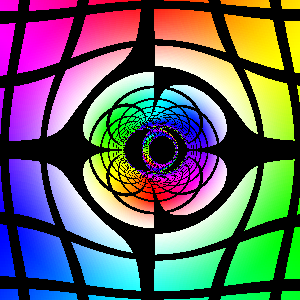
\includegraphics[width=.4\textwidth]{EqualMass_time8180.png}
		}
	\subfigure[$t = 3941$ M.]{
		\label{fig:eqm8190}
		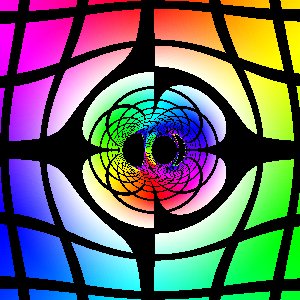
\includegraphics[width=.4\textwidth]{EqualMass_time8190.png}
		}
	\subfigure[$t = 3946$ M.]{
		\label{fig:eqm8200}
		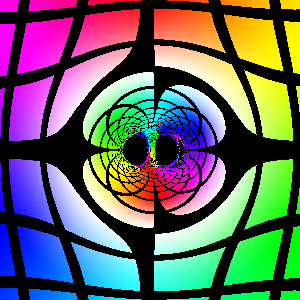
\includegraphics[width=.4\textwidth]{EqualMass_time8200.png}
		}
	\subfigure[$t = 3951$ M.]{
		\label{fig:eqm8210}
		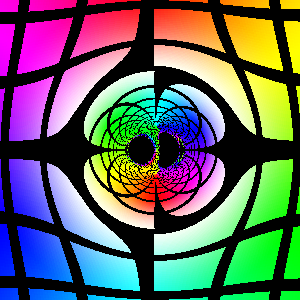
\includegraphics[width=.4\textwidth]{EqualMass_time8210.png}
		}
	\subfigure[$t = 3956$ M.]{
		\label{fig:eqm8220}
		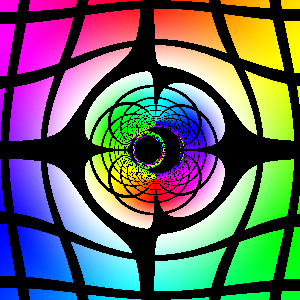
\includegraphics[width=.4\textwidth]{EqualMass_time8220.png}
		}
	\subfigure[$t = 3961$ M.]{
		\label{fig:eqm8230}
		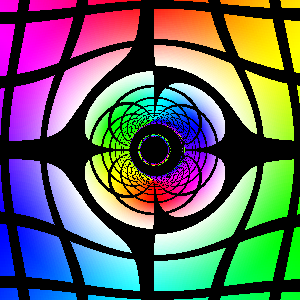
\includegraphics[width=.4\textwidth]{EqualMass_time8230.png}
		}
	\caption{Side view of a binary black hole inspiral before merger. Merger occurs at $t = 3910$ M but it has not yet been seen by the observer located $\approx50$ M away from the black holes. The angular momentum of the orbit in these images is upwards. The resolution of the observer's pinhole camera is $300 \times 300$.}
\end{figure}

In addition to the side view images, Fig. \ref{fig:eqmtop6580} shows a top-down view of the binary black hole system at $t = 3167$ M. The observer is placed 50 M away at the positive $z$-axis, i.e. $(x,y,z) \rightarrow (0,0,50)$, looking straight in the negative $z$-direction. At this time, the Einstein rings of the two black holes forms one oval Einstein ring. Interestingly, even though the angular momentum of the system is pointing out of the page, we do not see a significant tangential twisting of the lines inside the Einstein ring unlike the Kerr hole cases. The pattern of the lines inside the Einstein ring is particularly interesting and we will have to visualize the trajectories of the photons that make up that region to fully understand the features.

\begin{figure}[H]
   \centering
   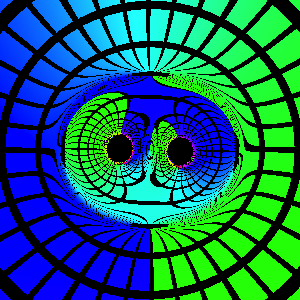
\includegraphics[width=.6\textwidth]{EqualMassTop_t6580.png} % requires the graphicx
   \caption{Top-down view of the equal mass non-spinning binary black hole system at $t = 3167$ M. The resolution of the pinhole camera is $300 \times 300$.}
   \label{fig:eqmtop6580}
\end{figure}

\newpage
\section{Conclusion}
In this report, we have presented a robust method of visualizing images distorted by one or more black holes. We have also shown that our method agrees well with direct integration from analytics. In addition, we have also produced some images of single black holes as well as binary black holes which show strong spacetime distortions.

We are currently working towards an adaptive camera routine where we will not have a uniform distribution of geodesics on the image. Instead, more geodesics will be integrated in areas which would have been under-resolved such as regions close to the black holes. Such adaptive camera routine will ensure that we have a high-resolution image in the shortest amount of computational time possible.
Future work will be devoted to including some astrophysically relevant quantities in the computation such as the redshift as well as the brightness light curves.

\section{Acknowledgements}
We would like to thank the following members of SXS collaboration who have been working with us throughout the project: Andrew Bohn (Cornell), William Throwe (Cornell), and Francois Hebert (Cornell). We would also like to thank the LIGO SURF program for their funding and support for the project.

\begin{thebibliography}{15}
\bibitem{krawisz} Krawisz, D. G., Black Hole Visualization and Animation, thesis, The University of Texas at Austin (2010).
%
\bibitem{lindner} Breen, \emph{et al.}, Invitation to embarassingly parallel computing, \emph{Am. J. Phys.}, \textbf{76}, 347--352 (2008).
%
\bibitem{scheel} Cohen, M. I., Preiffer, H. P. and Scheel, M. A., Revisiting Event Horizon Finders, \emph{Class. Quantum Grav.}, \textbf{26}, 035005 (2009).
%
\bibitem{shapiro} Shapiro, S. L. and Teukolsky, S. A., Gravitational collapse to neutron stars and black holes: Computer generation of spherical spacetimes, \emph{Astrophys. J.}, \textbf{235}:199--215 (1980).
%
\bibitem{hughes} Hughes, S. A., \emph{et al.}, Finding black holes in numerical spacetimes, \emph{Phys. Rev. D}, \textbf{49}, 4004--4015 (1994).
%
\bibitem{anninos} Anninos, P., \emph{et al.}, Dynamics of apparent and event horizons, \emph{Phys. Rev. Lett.} \textbf{74}, 630--633 (1995).
%
\bibitem{libson} Libson, J., \emph{et al.}, Event horizons in numerical relativity: Methods and tests, \emph{Phys. Rev. D}, \textbf{53}, 4335--4350 (1996).
%
\bibitem{bohn} Bohn, A., Building a new event horizon finder, \emph{Simulating eXtreme Spacetimes Video Conference} (2012).
%
\bibitem{mtw} Misner, C. W., Thorne, K. S. and Wheeler, J. A., \emph{Gravitation}, W. H. Freeman and Co., San Francisco pp. 570--577 (1973).
%
\bibitem{nichols} Nichols, D. A., \emph{et. al}, Visualizing spacetime curvature via frame-drag vortexes and tidal tendexes: General theory and weak-gravity applications, \emph{Phys. Rev. D}, \textbf{84}, 124014 (2011).
%
\bibitem{shadows} Yumoto, A., \emph{et. al.}, Shadows of Multi-Black Holes: Analytic Exploration, {\tt arXiv:1208.0635 [gr-qc]}.
%
\bibitem{gyoto} Vincent, F. H., \emph{et. al.}, 3+1 geodesic equations and images in numerical spacetimes, {\tt arXiv:1208.3927 [gr-qc]}.
\end{thebibliography}


\end{document}